\begin{figure}[p]
\centering
    \begin{subfigure}[t]{0.45\textwidth}
    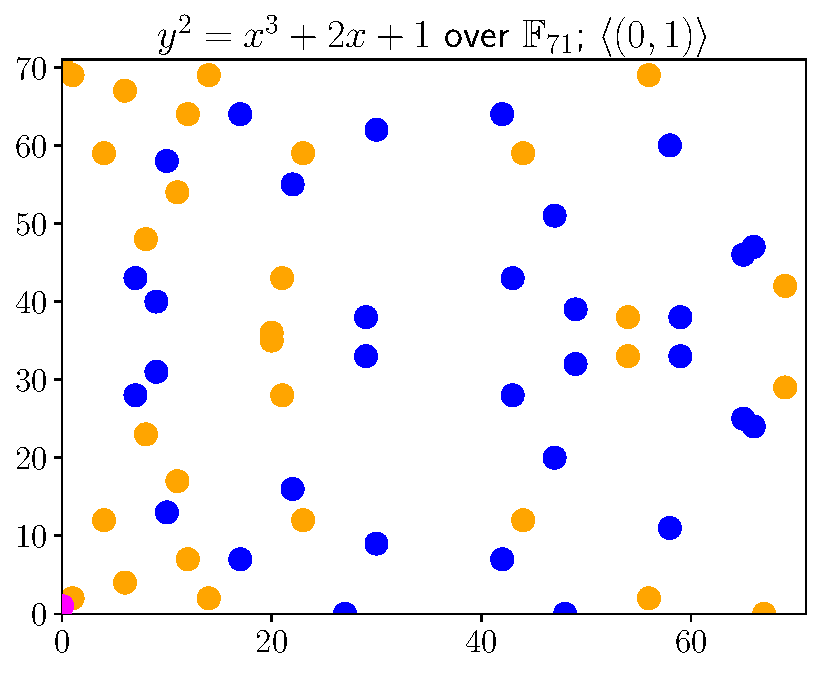
\includegraphics[width=\textwidth]{plots/ec_finite/ec_finite_F_71_2_1_subgroup_0_1.pdf}
    \caption{\textcolor{orange}{Subgroup} generated by
        $\color{magenta} \parens{0,1}$}
    \label{fig:ec_finite_plots_subgroups_0_1}
    \end{subfigure}
    \begin{subfigure}[t]{0.45\textwidth}
    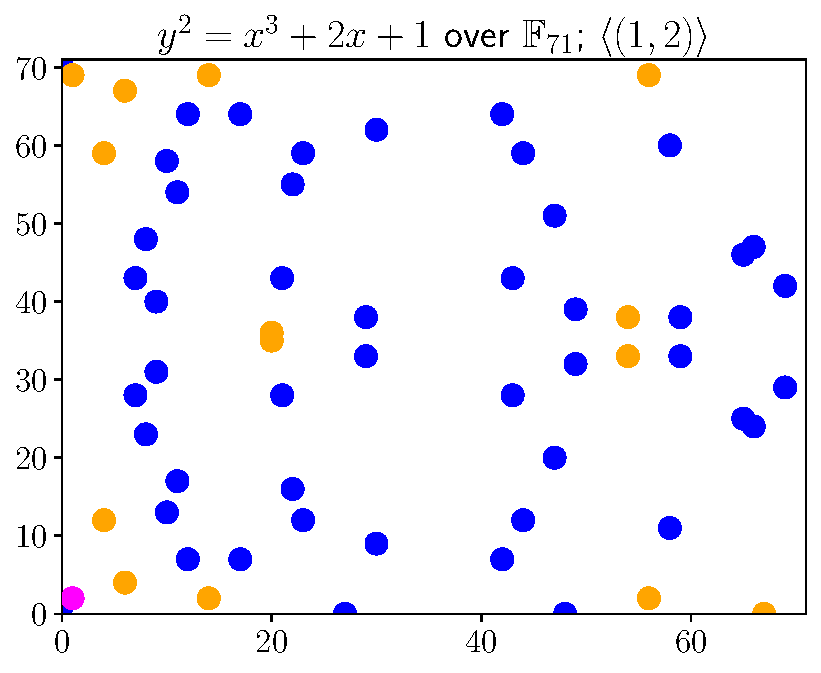
\includegraphics[width=\textwidth]{plots/ec_finite/ec_finite_F_71_2_1_subgroup_1_2.pdf}
    \caption{\textcolor{orange}{Subgroup} generated by
        $\color{magenta}\parens{1,2}$}
    \label{fig:ec_finite_plots_subgroups_1_2}
    \end{subfigure}

    \begin{subfigure}[t]{0.45\textwidth}
    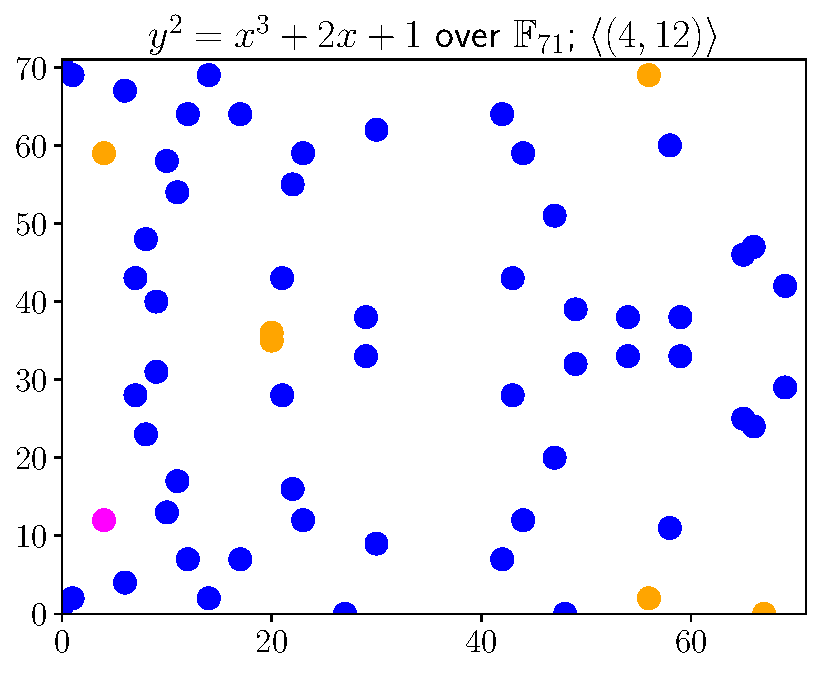
\includegraphics[width=\textwidth]{plots/ec_finite/ec_finite_F_71_2_1_subgroup_4_12.pdf}
    \caption{\textcolor{orange}{Subgroup} generated by
        $\color{magenta}\parens{4,12}$}
    \label{fig:ec_finite_plots_subgroups_4_12}
    \end{subfigure}
    \begin{subfigure}[t]{0.45\textwidth}
    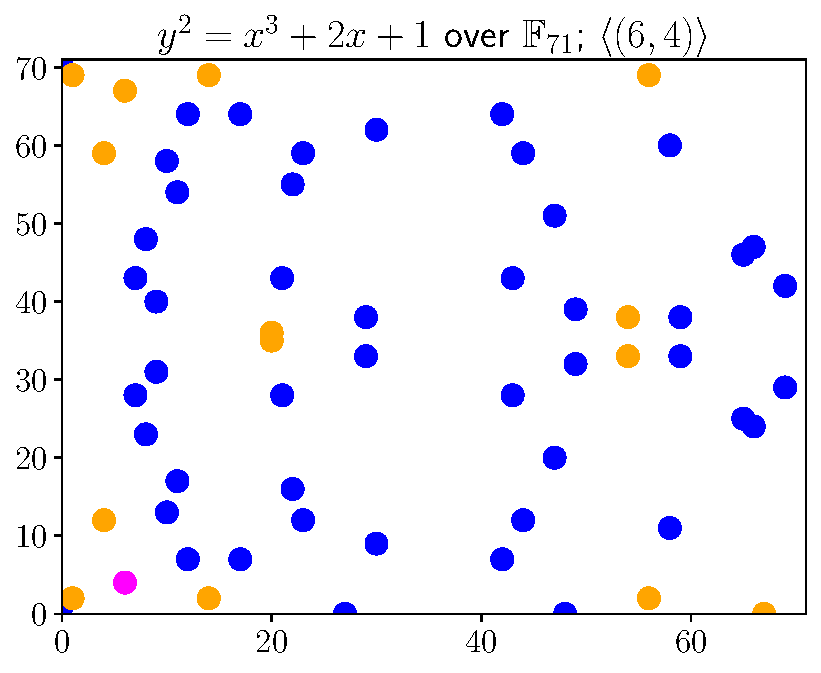
\includegraphics[width=\textwidth]{plots/ec_finite/ec_finite_F_71_2_1_subgroup_6_4.pdf}
    \caption{\textcolor{orange}{Subgroup} generated by
        $\color{magenta}\parens{6,4}$}
    \label{fig:ec_finite_plots_subgroups_6_4}
    \end{subfigure}

    \begin{subfigure}[t]{0.45\textwidth}
    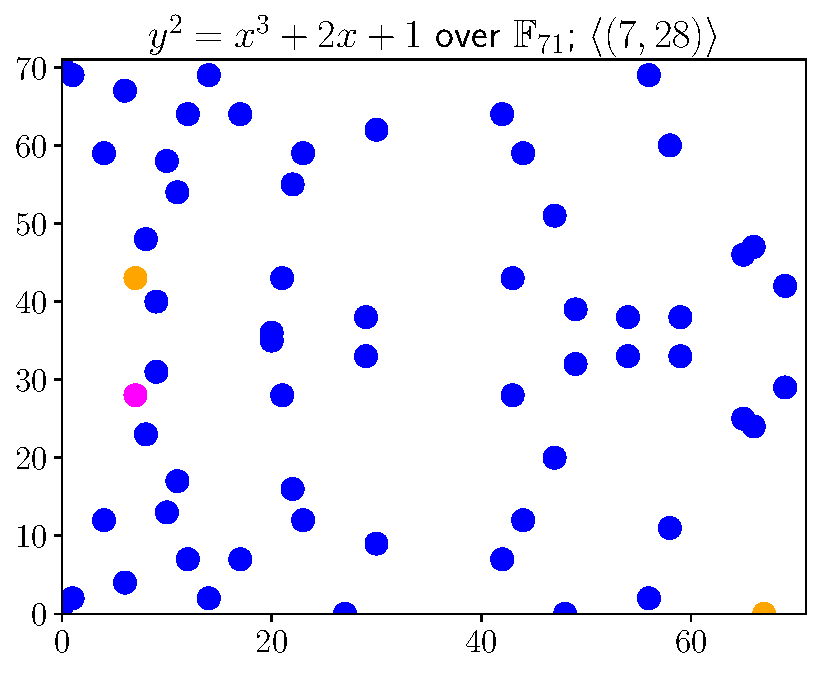
\includegraphics[width=\textwidth]{plots/ec_finite/ec_finite_F_71_2_1_subgroup_7_28.pdf}
    \caption{\textcolor{orange}{Subgroup} generated by
        $\color{magenta}\parens{7,28}$}
    \label{fig:ec_finite_plots_subgroups_7_28}
    \end{subfigure}
    \begin{subfigure}[t]{0.45\textwidth}
    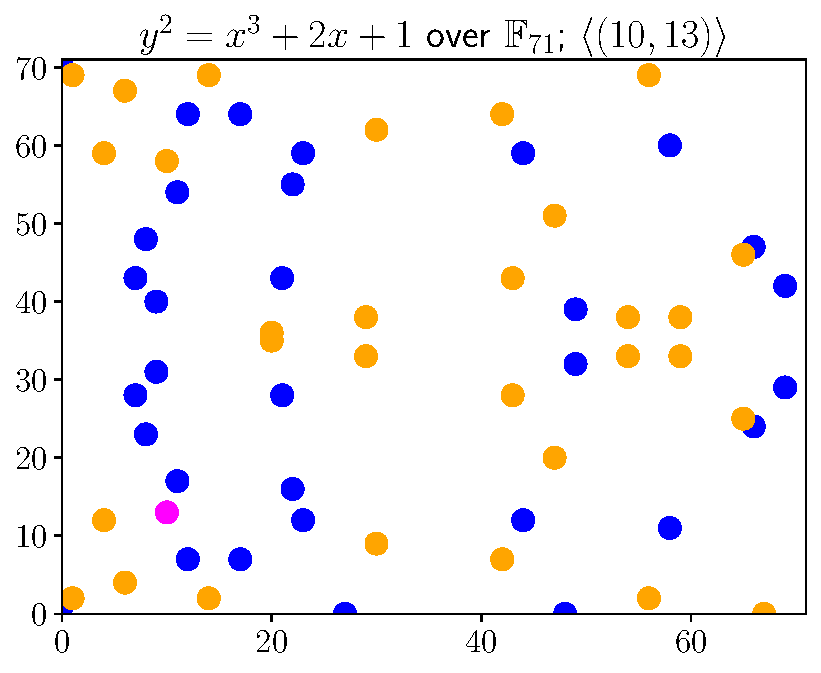
\includegraphics[width=\textwidth]{plots/ec_finite/ec_finite_F_71_2_1_subgroup_10_13.pdf}
    \caption{\textcolor{orange}{Subgroup} generated by
        $\color{magenta}\parens{10,13}$}
    \label{fig:ec_finite_plots_subgroups_10_13}
    \end{subfigure}
    \caption[Plots of subgroups of elliptic curves over finite fields]{Here
        are plots of \glspl{elliptic curve} over $\F_{71}$.
        The \glspl{elliptic curve} are all the same: $y^{2} = x^{3} + 2x + 1$.
        In each plot, we also show different cyclic subgroups;
        \textcolor{orange}{subgroups} generated by different
        \textcolor{magenta}{base points}.}
    \label{fig:ec_finite_plots_subgroups}
\end{figure}
